\documentclass{beamer}

\usecolortheme[light]{solarized}

\beamertemplatenavigationsymbolsempty


\usepackage{booktabs}
\usepackage{graphicx}
\usepackage{hyperref}
\usepackage{minted}
\usepackage{moresize}
\usepackage{centernot}
\usepackage{standalone}
\usepackage{tcolorbox}
\usepackage{tikz}
\usepackage[normalem]{ulem}
\usepackage{xpatch}
\usepackage{fix-cm}

\xpatchcmd{\sout}
  {\bgroup}
    {\bgroup\def\ULthickness{2pt}}
      {}{}

\usetikzlibrary{calc, patterns}
\usetikzlibrary{arrows}
\usetikzlibrary{decorations.markings}
\usetikzlibrary{decorations.text}

\definecolor{twitter}{RGB}{64, 153, 255}
\definecolor{github}{RGB}{211, 211, 211}

\newcommand{\assetsfolder}{./assets}
\newcommand{\revisitresearchfolder}{$HOME/rsc/revisiting-axelrod-second}
\newcommand{\moranresearchfolder}{$HOME/rsc/axelrod-moran}
\newcommand{\mlresearchfolder}{$HOME/rsc/ml-paper}

\begin{document}

    \begin{frame}
        \begin{center}
            \Huge
                Reproducing Research on Cooperation

               \vfill

            \Large
               Vince: \href{https://twitter.com/drvinceknight}{@drvinceknight}\\
        \end{center}

        % Thank you very much ...  My name is Vince Knight and it's a true pleasure
        % to be speaking here today. Thank you to Marc Harper for the
        % invitation. I'll be speaking to you today about 3 topics that are
        % linked.
    \end{frame}

    \begin{frame}
               \begin{columns}
                   \begin{column}{.45\textwidth}
                       \begin{center}
                       \includegraphics[height=3cm]{\assetsfolder/CUident_CMYK.eps}
                       \end{center}

                       \begin{center}
                       \includegraphics[height=3cm]{\assetsfolder/axelrod_logo.png}
                       \end{center}
                   \end{column}
                   \begin{column}{.45\textwidth}
                       \begin{center}
                       \includegraphics[height=3cm]{\assetsfolder/ssi-logo.png}
                       \end{center}

                       \pause
                       \begin{center}
                       \includegraphics[trim={15cm 0 0 0}, clip, height=3cm]{\assetsfolder/discdog.jpg}
                       \end{center}
                   \end{column}
               \end{columns}

        % Notes I am an associate professor at Cardiff University's School of
        % Mathematics where I teach game theory and computer programming.
        % It's the job I wanted all my life and I'm super lucky to get to
        % teach things I'm passionate about.  I am also a fellow of the
        % Sustainable Software Institute: I'll
        % speak more about this institute at the correct time.  I am also one of
        % the core developers of a Python library called the Axelrod
        % project and again: I'll speak about that at the relevant time
        % in this talk.  Finally, [click], in my free time I like to
        % throw plastic around for my dog: this is not at all relevant to
        % this talk.
    \end{frame}

    \begin{frame}
        \begin{center}
            \includegraphics[width=.7\textwidth]{\assetsfolder/nik_and_i.jpg}
        \end{center}
    \end{frame}

    \begin{frame}
    \begin{center}
        \href{https://www.bbc.co.uk/news/technology-54423988}{\includegraphics[width=.85\textwidth]{\assetsfolder/excel-error-causes-wrong-covid-count.png}}
        \end{center}

        % TODO write notes
    \end{frame}

	\begin{frame}
		\begin{center}
			\includegraphics[width=.7\textwidth]{\assetsfolder/lizard-tweet.png}
		\end{center}
		\begin{center}
			\pause
			\includegraphics[width=.35\textwidth]
			{\assetsfolder/lizard-cooperation.jpg}
		\end{center}

        % This is a tweet I specifically liked. The idea going on here (I
        % believe), is that we want to study if a specific Lizard is going to
        % dominate another. Perhaps this gets correlated to some genetic marker
        % or even prior behaviour.

        % The reason I like this tweet, is that it is a nice illustration of
        % game theory. Game theory is the study of outcomes based on behaviour
        % in rule based systems. So for example: the lizard that was not fed is
        % more likely to fight and win the warm part of the coop perhaps?

        % [CLICK] Here is the output

        % And the reason this tweet is cool is because it evidences the need for
        % the subject: sometimes out of simple systems we do not get the
        % behaviour we expect. Indeed, here cooperative behaviour has emerged.

	\end{frame}

	\begin{frame}
		\fontsize{74}{65}\selectfont
		\begin{center}
			\(
				\begin{pmatrix}
					3 & 0\\
					5 & 1
				\end{pmatrix}
			\)
		\end{center}

        % A well used game (set of rules) is the Prisoners Dilemma. You might
        % have heard of this game before, the general concept is that you have
        % the option to cooperate or defect when encountering someone else.
        % Cooperation is essentially the selfish action: giving a bit to ensure
        % the individual you encounter gains more. Defection on the other hand
        % is the selfish action: take whatever you can.
        % When both cooperate it's good for both (for example the lizards).
	\end{frame}


    \begin{frame}
		\begin{center}
            (Slide used at PyCon 2015)
			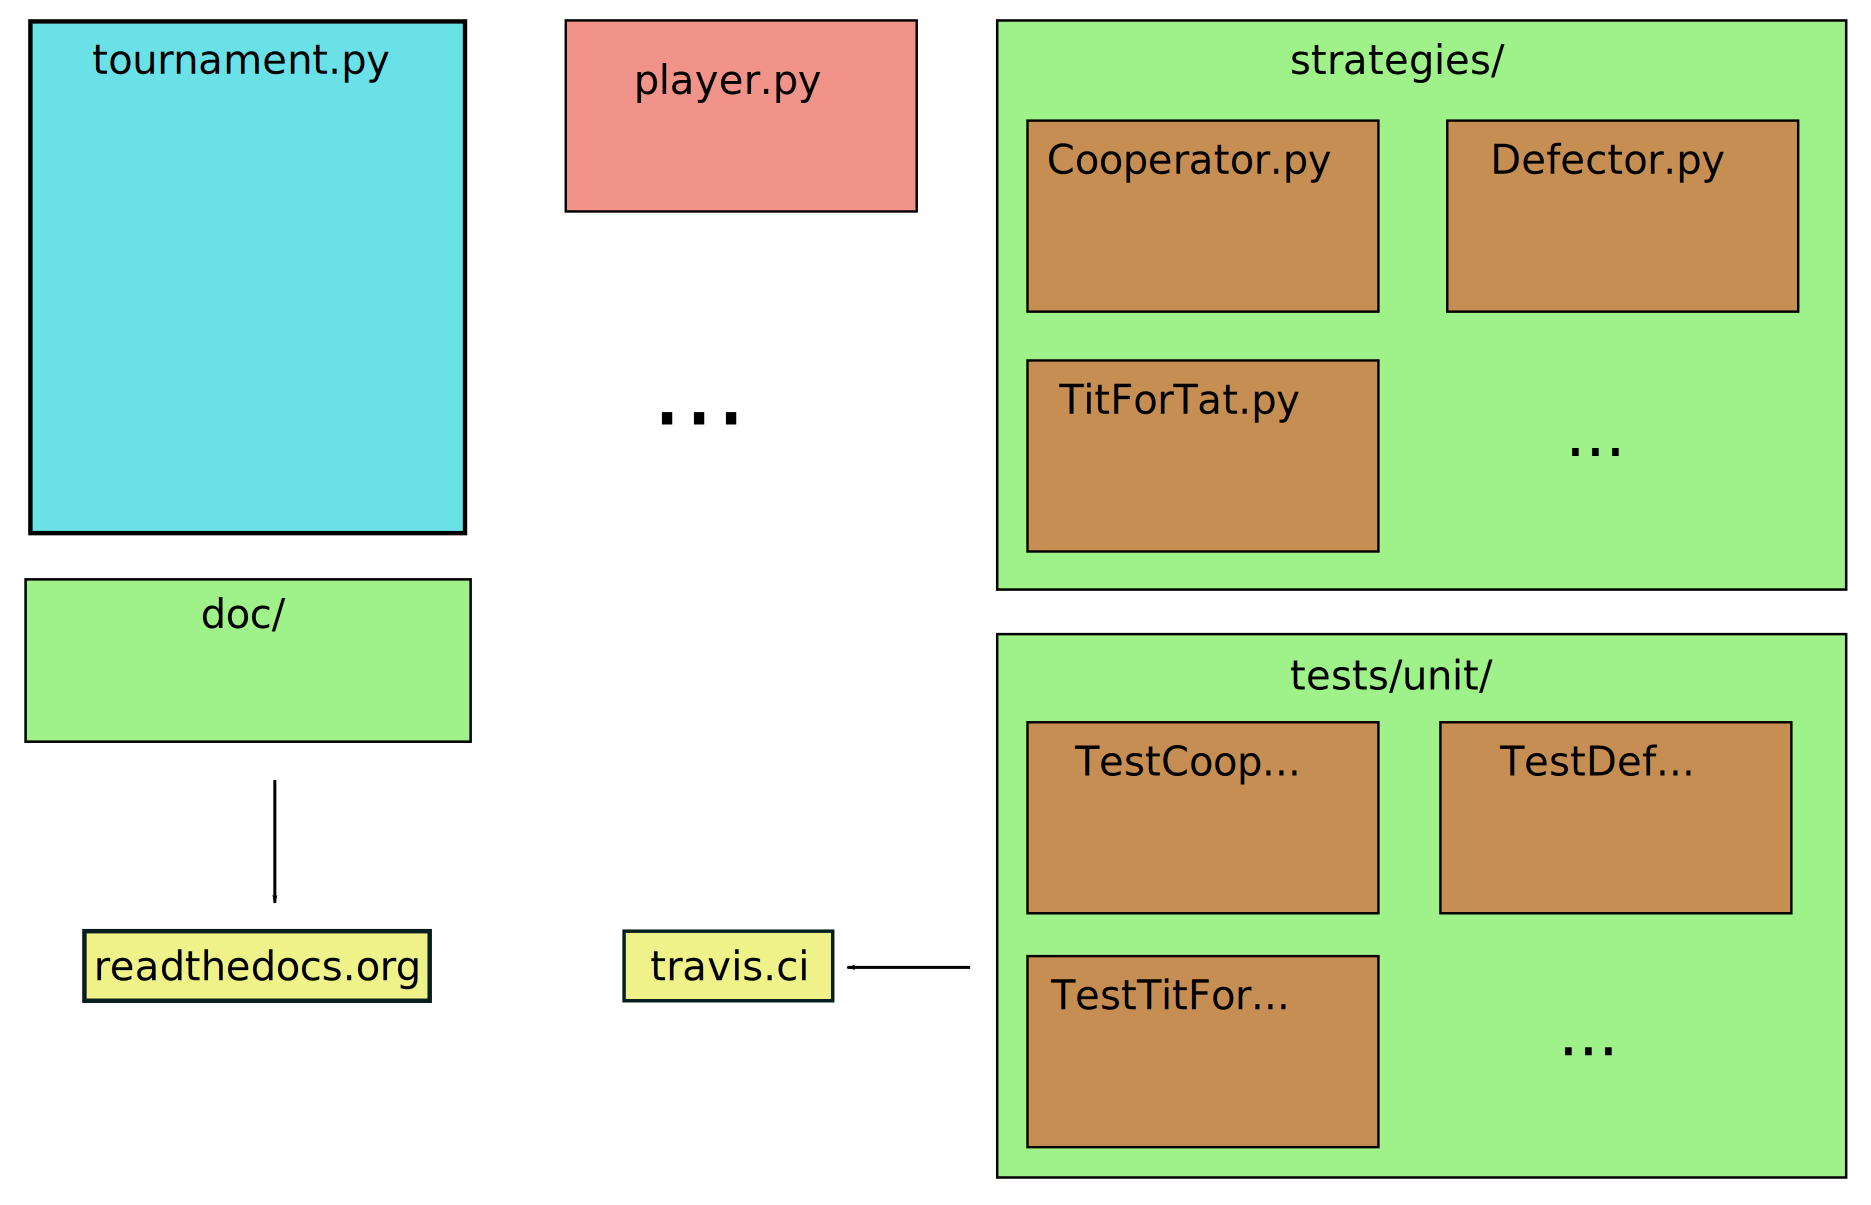
\includegraphics[width=.9\textwidth]{\assetsfolder/outline_of_library.pdf}
		\end{center}
    \end{frame}

    \begin{frame}
    \begin{center}
        \href{https://journals.sagepub.com/doi/abs/10.1177/002200278002400101}{Axelrod, Robert. "Effective choice in the prisoner's dilemma." Journal of conflict resolution 24.1 (1980): 3-25.}
        \end{center}

        % TODO write notes
    \end{frame}

    \begin{frame}
		\begin{center}
            \includegraphics[height=.85\textwidth]{\assetsfolder/axelrod_second_all_ranks.png}
		\end{center}
        % TODO Write notes with explanation.
    \end{frame}

    \begin{frame}
		\begin{center}
            \includegraphics[height=.85\textwidth]{\assetsfolder/axelrod_second_number_of_wins.png}
		\end{center}
        % TODO Write notes with explanation.
    \end{frame}

    \begin{frame}

        \begin{center}
            \Huge
            \[
                \text{Ambiguous description}
            \]
            \[
                \centernot\implies
            \]
            \[
                \text{Clear results}
            \]
        \end{center}

        % TODO write notes
    \end{frame}

    \begin{frame}
    \begin{center}
        \includegraphics[width=.85\textwidth]{\assetsfolder/email_from_axelrod.png}
        \end{center}

        % TODO write notes
    \end{frame}

    \begin{frame}
    \begin{center}
        \href{https://journals.sagepub.com/doi/abs/10.1177/002200278002400301}{Axelrod, Robert. "More effective choice in the prisoner's dilemma." Journal of conflict resolution 24.3 (1980): 379-403.}
        \end{center}

        % TODO write notes
    \end{frame}

\begin{frame}[fragile]{}
    \begin{minted}{fortran}
      FUNCTION K92R(J,M,K,L,R, JA)
    C BY ANATOL RAPOPORT
    C TYPED BY AX 3/27/79 (SAME AS ROUND ONE TIT FOR TAT)
    c replaced by actual code, Ax 7/27/93
    c  T=0
    c   K92R=ITFTR(J,M,K,L,T,R)
      k92r=0
      k92r = j
    c test 7/30
    c   write(6,77) j, k92r
    c77   format(' test k92r. j,k92r: ', 2i3)
      RETURN
      END
        \end{minted}

        % Here is what some of the original code: this is Tit For Tat. Written
        % in Fortran.
\end{frame}

    \begin{frame}
    \begin{center}
        \scalebox{.8}{
            \includestandalone{assets/strategy_diagram}
                     }
    \end{center}
    \end{frame}

    \begin{frame}
        \begin{center}
            \includegraphics[width=\textwidth]{\revisitresearchfolder/assets/original_tournament_rankings_all_approaches.pdf}
        \end{center}

        % But even with the code: it is difficult to reproduce the work. This is
        % a number of different ways of computing the results and they do not
        % all match. There could be a number of reasons for this, slightly
        % different compilers: not the EXACT same code. The main conclusions
        % though: do match up. The simple strategy Tit For Tat wins.
    \end{frame}

    \begin{frame}
        \begin{center}
            \includegraphics[width=\textwidth]{\revisitresearchfolder/assets/original_tournament_with_extra_strategy_ranks_vs_library_ranks.pdf}
        \end{center}

        % The library has had a number of strategies contributed. We can
        % investigate if one would have changed the results and impressively:
        % no! Tit For Tat still wins.
    \end{frame}

    \begin{frame}
        \begin{center}
            \includegraphics[width=.7\textwidth]{\revisitresearchfolder/assets/full_tournament_pairwise_cooperation_rates.pdf}
        \end{center}

        % However if we run a tournament with all available strategies (the size
        % is too big here) then Tit for Tat no longer wins. The tournament is
        % won by much more complex strategies and what this plot shows here is,
        % is that they all cooperate with each other and/or don't with the lower
        % ranking strategies.
    \end{frame}

    \begin{frame}

        \begin{center}
            \Huge
            \[
                \text{Available code}
            \]
            \[
                \centernot\implies
            \]
            \[
                \text{Exact results}
            \]
        \end{center}

        % TODO write notes
    \end{frame}


    \begin{frame}
        \begin{center}
            \href{}{\includegraphics[width=.7\textwidth]{\assetsfolder/please-download-the-postdoc-tweet.png}}
        \end{center}

        % Simply "putting code up" is sadly not a solution. Even though at times
        % it's progress.
    \end{frame}

    \begin{frame}
        \begin{center}
            \Huge What do we do?
        \end{center}
        \pause
        \begin{center}
            \includegraphics[width=.7\textwidth]{\assetsfolder/elmo-fire.jpg}
        \end{center}

        % Simply "putting code up" is sadly not a solution. Even though at times
        % it's progress.
    \end{frame}

    \begin{frame}
        \begin{center}
            \href{https://twitter.com/betatim/status/1004077975233552385}{\includegraphics[width=.7\textwidth]{\assetsfolder/ms-github-importance-of-archiving-tweet.png}}
        \end{center}
        % The recent MS + Github saw a number of hot takes. This one in
        % particular I thought was quite good. The problem associated with "just
        % putting your code up" isn't as simple as being able to run it and/or
        % understand it. There are fundamental problems associated to making
        % sure that software is actually there! And that it was/is the software
        % that was actually used to do the research.
    \end{frame}

    \begin{frame}
        \begin{center}
            \href{https://twitter.com/JamesCampbell95/status/996419422951825410}{\includegraphics[width=.7\textwidth]{\assetsfolder/blockchain-instead-of-archiving-tweet.png}}
        \end{center}

        % There are some great technological solutions: this tweet from a PhD
        % student at Cardiff is 1/4 describing a paper that uses blockhain to
        % ensure archival of all materials.
    \end{frame}

    \begin{frame}
        \begin{center}
            \href{https://twitter.com/legogradstudent/status/979776951517876225}{\includegraphics[width=.7\textwidth]{\assetsfolder/just-use-git-tweet.png}}
        \end{center}

        % This is a slightly worse to this: tooling is not the only solution
        % (to be clear: this is not a blockchain talk)
        % Just telling people to use tools is not sufficient.
    \end{frame}

	\begin{frame}
		\begin{center}
			\begin{tikzpicture}

				\node [font=\large, draw] (technology) at (-4, 4.5) {Technology};
				\node [font=\large, draw] (culture) at (4, 3.5) {Culture};

				\draw [very thick] (0, 0) -- (0, 6);
				\draw [very thick] (-2, 0) -- (2, 0);

				\draw [very thick] (-4, 6.5) -- (4, 5.5);
				\draw [very thick] (-4, 6.5) -- (technology);
				\draw [very thick] (4, 5.5)  -- (culture);
			\end{tikzpicture}
		\end{center}

        % We need to talk about balancing technology with culture. There are a
        % number of things happening in that sense.
	\end{frame}

	\begin{frame}
	   \begin{center}
		   \includegraphics[height=6cm]{\assetsfolder/ssi-logo.png}

			\url{https://www.software.ac.uk/}
	   \end{center}

       % The Sustainable Software Institute, is an organisation in the UK that
       % is funded by one of the main research funders and aims to promote
       % better practice in research.

       % One of the many things they do is run a fellowship programme: every
       % year a number of individuals are selected (in quite a competitive
       % environment) to be (lifelong) fellows with goals to spread best
       % practice. For example a PhD student of mine is using his fellowship to
       % give talks and produce learning resources in Welsh (Wales is a bi
       % lingual country).

       % As well as this, the SSI, run a yearly workshop (an unconference) which
       % brings together people from a number of academic fields to discuss and
       % improve the landscape of software in research.
       % Some examples that directly come out of this workshop include `recipy`
       % a Python library that automatically builds up a database of what code
       % ran to produce every output.
	\end{frame}

	\begin{frame}
	   \begin{center}
		   \includegraphics[height=7cm]{\assetsfolder/UKRSE-logo.png}

			\url{http://rse.ac.uk/}
	   \end{center}

       % Another output is the notion of a research software engineer. They're
       % adamant that anyone who write code and does research is an rse but
       % we're seeing a number of groups arise around the world: with scientists
       % whose role it is to contribute (through writing of software) to the
       % research being done.
    \end{frame}

	\begin{frame}
	   \begin{center}
           \includegraphics[width=6cm]{\assetsfolder/joss-logo.png}

			\url{http://joss.theoj.org/}
	   \end{center}

       % TODO Discuss https://twitter.com/danielskatz/status/1351879941932134402

       % We have to ask ourselves what is one of the main reasons for poor
       % practice. I believe, in part because it's good enough. Most
       % promotion/tenure like procedures do not (YET) recognise software.
       % There is ongoing work to recognise software as a research contribution.
       % For example JOSS: a completely open journal. These are short papers
       % that, usually if a piece of code has been written correctly (tested,
       % documented, etc), take very little effort to write.
	\end{frame}

	\begin{frame}
	   \begin{center}
		   \includegraphics[width=8cm]{\assetsfolder/the-carpentries-logo.pdf}

			\url{https://carpentries.org/}
	   \end{center}

       % The problem is of course subtle, some of you might have heard of
       % Software carpentry. The carpentries encompasses that as well as what
       % was called the library and data carpentries. These are a collection of
	   % workshops  that aim to introduce researchers to the why and how of best
	   % practice.
	\end{frame}

    \begin{frame}
    \begin{center}
        \scalebox{.8}{
            \includestandalone{assets/best_practices_triangle}
                     }
    \end{center}
    \end{frame}

	\begin{frame}
		\Huge
		\begin{center}
			\textit {For example...}
		\end{center}

        % I'm going to give an example of some of the things I've spoken about
        % here.
	\end{frame}


    \begin{frame}
  \begin{block}{}
  Knight, Vincent Anthony, et al. ``An open framework for the
        reproducible study of the iterated prisoner's dilemma." Journal of Open
        Research Software 4.1 (2016).
  \end{block}
        \begin{center}
            \includegraphics[width=.9\textwidth]{\assetsfolder/first_paper_tournament.pdf}
        \end{center}
    \end{frame}

    \begin{frame}
  \begin{block}{}
    Harper, Marc, et al. ``Reinforcement learning produces dominant strategies for the Iterated Prisoner’s Dilemma." PloS one 12.12 (2017): e0188046.
  \end{block}
        \begin{center}
            \includegraphics[width=.65\textwidth]{\assetsfolder/FSM16.pdf}
        \end{center}
    \end{frame}
    
    \begin{frame}
        \begin{center}
            \includegraphics[width=.65\textwidth]{\assetsfolder/cooperation_0_0_10000_Evolved_FSM_16_array.pdf}
        \end{center}
    \end{frame}

    \begin{frame}
  \begin{block}{}
Knight, Vincent, et al. ``Evolution reinforces cooperation with the emergence of self-recognition mechanisms: An empirical study of strategies in the Moran process for the iterated prisoner’s dilemma." PloS one 13.10 (2018): e0204981.
  \end{block}
    \begin{center}
        \scalebox{.45}{
            \includestandalone{assets/fsm_one}
                     }
    \end{center}
    \end{frame}

    \begin{frame}
        \Huge
        \begin{center}
            Some conclusions
        \end{center}
    \end{frame}

    \begin{frame}
        \Huge
        \begin{center}
            Code should (verifiably) do what you think it does.
        \end{center}
    \end{frame}

    \begin{frame}
        \Huge
        \begin{center}
            Open code makes for better research.
        \end{center}
    \end{frame}


\begin{frame}
    \begin{footnotesize}
        \begin{tcolorbox}[colback=github,colframe=blue!40!black,title=
                Julie Rymer - \href{https://gitter.im/Axelrod-Python/Axelrod?at=591388592b926f8a6741435d}
                {@Chadys} - (10 May 2017):
    ]
                And I really wanted to thank you all, I discovered your project because of a
                course where we needed to participate in an open source project, and I had the
                occasion to compare the welcome me and my coworkers received here compared to
                other people from my class who worked on different project. And I've got to said
                you are awesome on that part and on the help your provide to newbies  I like
                your project so I'll try to continue to contribute now and then !
       \end{tcolorbox}
    \end{footnotesize}

   \begin{columns}
        \begin{column}{.35\textwidth}
            \begin{itemize}
                \item \href{https://twitter.com/NikoletaGlyn}{@NikoletaGlyn}
                \item \href{https://twitter.com/opcampbell}{@opcampbell}
                \item \href{http://marcharper.codes/}{marcharper.codes}
            \end{itemize}
        \end{column}
        \begin{column}{.65\textwidth}
            \begin{itemize}
                \item \href{https://github.com/Axelrod-Python/Axelrod}{github.com/Axelrod-Python/Axelrod}
                \item \href{https://axelrod.readthedocs.io/en/stable/}{axelrod.readthedocs.io}
            \end{itemize}
        \end{column}
   \end{columns}

        \begin{center}
               \href{https://twitter.com/drvinceknight}{@drvinceknight}
        \end{center}

   \begin{columns}
        \begin{column}{.5\textwidth}
            \begin{itemize}
                \item
                    \href{https://www.software.ac.uk/}{software.ac.uk}
                \item
                    \href{http://rse.ac.uk/}{rse.ac.uk}
            \end{itemize}
        \end{column}
        \begin{column}{.5\textwidth}
            \begin{itemize}
            \item
                \href{https://carpentries.org/}{carpentries.org}
            \item
                \href{http://joss.theoj.org/}{joss.theoj.org}
            \end{itemize}
        \end{column}
    \end{columns}
\end{frame}


\end{document}
